\section{Data Preprocessing}
\begin{frame}{}
  \Huge
  \centering
  \textbf{Data Preprocessing} \\
  \normalsize
  \vspace{1em}
  \textbf{Fashionopedia Dataset}
  \normalsize
\end{frame}

\begin{frame}{Removing Invalid Bounding Boxes}
  \textbf{Problem:} Some bounding boxes have zero width or height.

  \textbf{Solution:}
  \begin{itemize}
      \item Detect and remove invalid bounding boxes.
      \item Retain only boxes with positive area, along with their IDs, categories, and area values.
  \end{itemize}

  \begin{block}{}
  \textbf{Significance: }Invalid bounding boxes introduce noise and hurt model training.
  Cleaning at this stage ensures better stability and learning quality.
  \end{block}

  \begin{block}{}
    \textbf{Result: }Train and validation datasets maintain \textbf{45,623} and \textbf{1,158} images, respectively, but with only valid boxes.
  \end{block}
  \end{frame}

\begin{frame}{Visualizing Class Occurrences}

\begin{figure}[H]
    \centering
    \includegraphics[width=0.75\textwidth]{../report_final/images/classes.png}
\end{figure}

\end{frame}

\begin{frame}{Data Augmentation}
\small
We used Albumentations Library to do some data augmentation on the dataset.
\begin{block}{}
  \textbf{Significance: }Data augmentation boosts diversity, reduces overfitting,
  and improves generalization across different object appearances and conditions.
\end{block}

\small
\vspace{1.25em}
\centering
\begin{minipage}{0.78\textwidth}
  \textbf{Training Dataset:}
  \vspace{-0.25em}
  \begin{itemize}
    \setlength\itemsep{-0.25em}
    \item \textbf{Resize and Pad:} $500\times500$ px size.
    \item \textbf{Horizontal Flip:} $p=0.5$ for left-right invariance.
    \item \textbf{Brightness/Contrast Adjustments}.
    \item \textbf{Small Rotations and Scaling}.
    \item \textbf{Gaussian Blur and Noise}.
  \end{itemize}
\end{minipage}

% \begin{figure}[H]
%     \centering
%     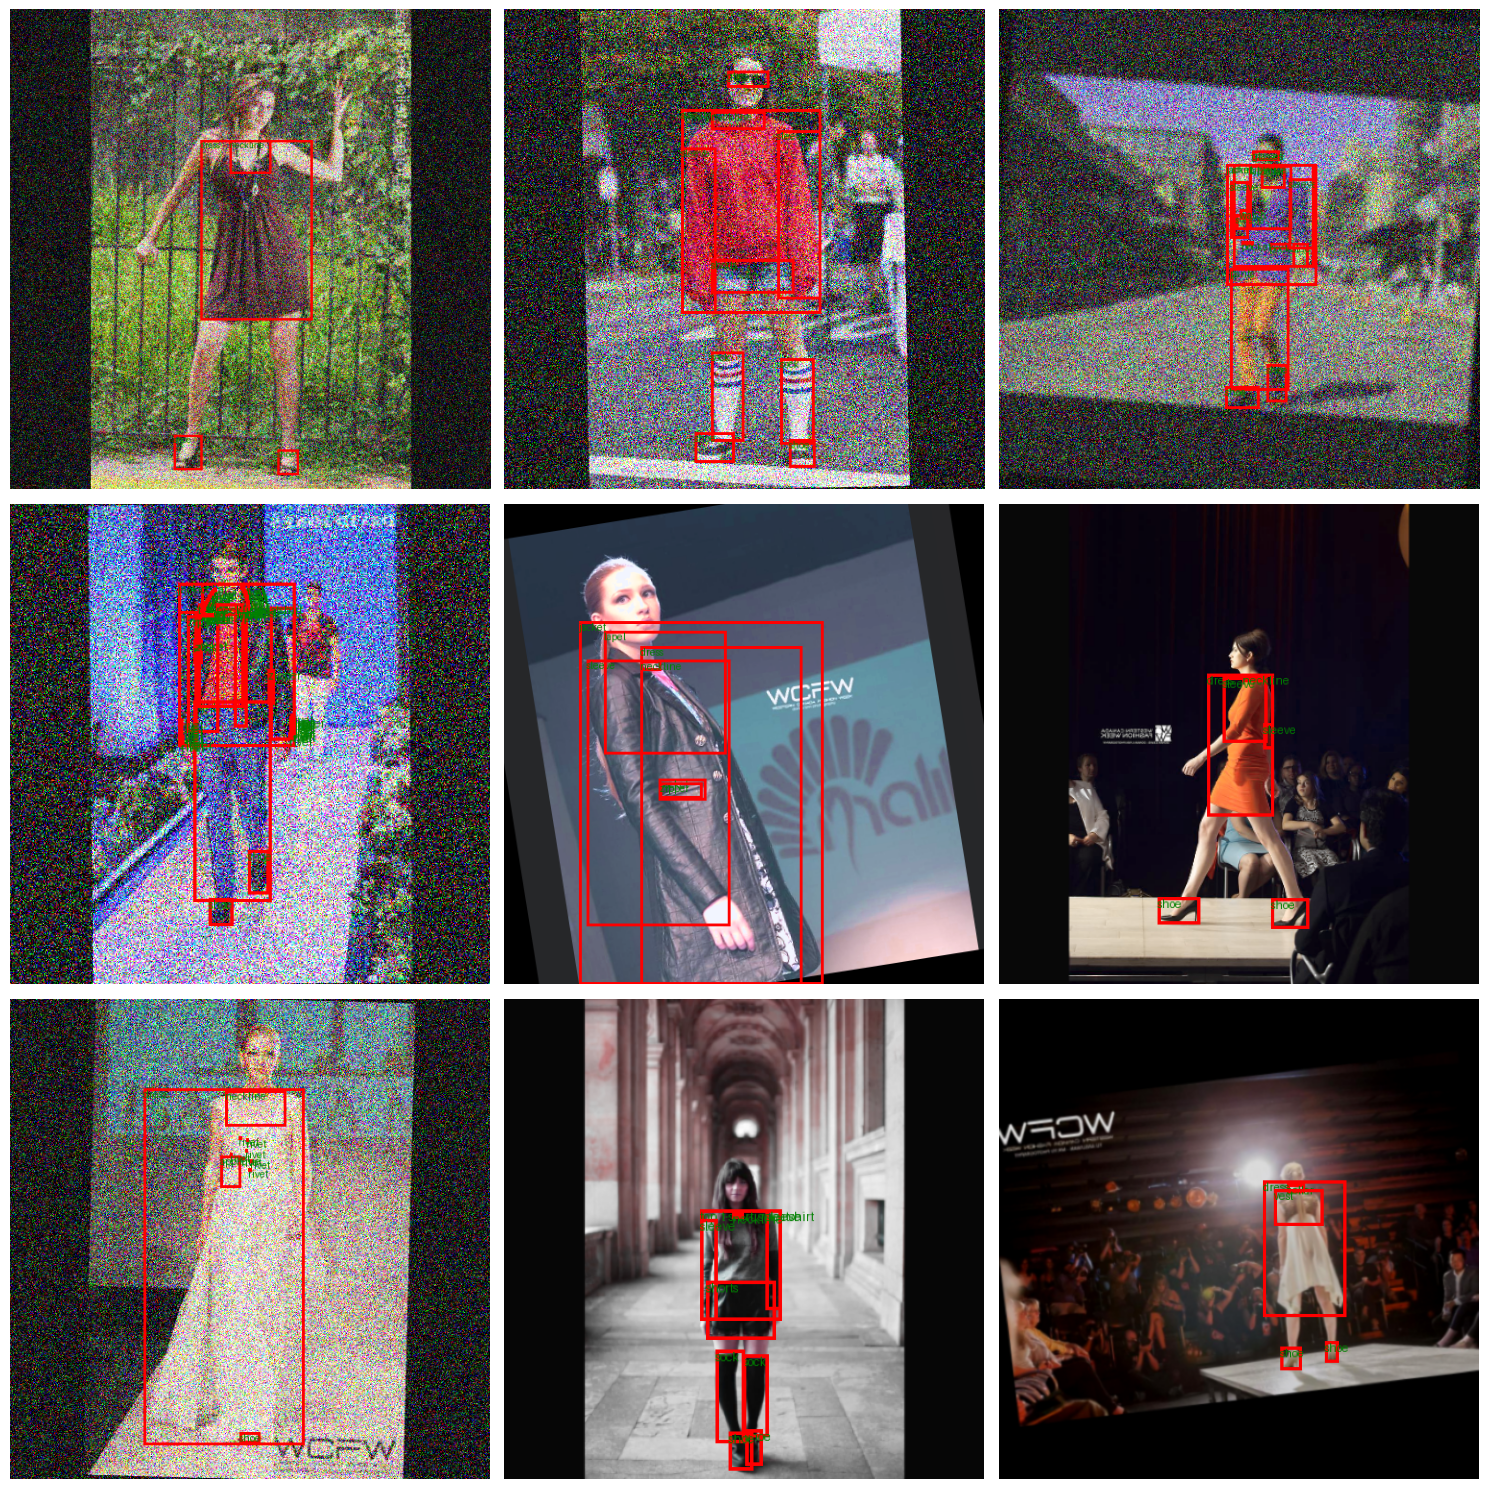
\includegraphics[width=0.75\textwidth]{images/augmented.png}
%     \caption{Example of augmented training images}
% \end{figure}
\end{frame}


\begin{frame}{Before Augmentation}

\begin{figure}[H]
    \centering
    \includegraphics[width=0.65\textwidth]{images/before_augmented.png}
\end{figure}

\end{frame}

\begin{frame}{After Augmentation}

\begin{figure}[H]
    \centering
    \includegraphics[width=0.65\textwidth]{images/after_augmented.png}
\end{figure}

\end{frame}

\begin{frame}{Feature Extraction}
\begin{minipage}{0.68\textwidth}
    PIL images need to be converted into numerical tensors for training.

    \vspace{1em}
    \textbf{Tool Used:}
    YOLOS Feature Extractor (pretrained; applies normalization, standardization)

    \vspace{0.75em}
    \begin{block}{}
      \textbf{Significance: }Feature extractors prepare raw images into consistent formats,
      allowing models to focus on learning patterns, not on raw inconsistencies.
    \end{block}
  \end{minipage}
\hfill
\begin{minipage}{0.25\textwidth}
    \centering
    \includegraphics[width=0.9\linewidth]{../report_final/images/yolos.png}

    \vspace{0.5em}
    \small Image after YOLOS feature extraction
\end{minipage}
\end{frame}


\begin{frame}{}
  \Huge
  \centering
  \textbf{Data Preprocessing} \\
  \normalsize
  \vspace{1em}
  \textbf{Fashion Product Images Dataset}
  \normalsize
\end{frame}

\begin{frame}{Fashion Product Images Dataset Cleaning}
  \textbf{Preprocessing Steps:}
  \begin{enumerate}
      \item<1-> Remove duplicate entries.
      \item<2-> Exclude ``Unknown'' product groups.
      \item<3-> Filter out descriptions longer than 40 words. Since FashionCLIP has a token limit of 77, this ensures safety margins.
      \item<4-> Remove rare product types (less than 10 samples).
      \item<5-> Assign random prices to each item.
  \end{enumerate}

  \begin{block}<6->{}
    \textbf{Result: }Dataset reduced from \textbf{105,542} to \textbf{37,704} entries.
  \end{block}
\end{frame}